\section{\label{sec:operation}Symmetry operation and space group}

\subsection{Affine group}

\subsubsection{Lattice}

\begin{screen}
  \begin{defn}[lattice]
    \textit{Lattice} $L$ in $\mathbb{R}^{n}$ is the set spanned by $n$ independet vectors $\bm{a}_{1}, \dots, \bm{a}_{n}$ as
    \begin{align}
      L \coloneqq \set{ \sum_{i=1}^{n} l_{i} \bm{a}_{i} }{ l_{1}, \dots, l_{n} \in \mathbb{Z} }.
    \end{align}
    These vectors $\bm{a}_{1}, \dots, \bm{a}_{n}$ are called \term{lattice basis} of $L$.
  \end{defn}
\end{screen}

We introduce the standard inner product in vector space $\mathbb{R}^{n}$.
Then it is convenient to define the following matrix for calculating distances.

\begin{screen}
  \begin{defn}[metric tensor]
    Let $\mathbf{A} \coloneqq ( \mathbf{a}_{1}, \cdots, \mathbf{a}_{n} )$ be basis vectors of a lattice $L$.
    A \term{metric tensor} of $L$ is
    \begin{align}
      \bm{G} \coloneqq \bm{A}^{\top} \bm{A}.
    \end{align}
  \end{defn}
\end{screen}

We remark that metric tensor $\bm{G}$ implicitly depends on the choice of basis vectors of $L$.
When basis vectors are changed from $\bm{A}$ to $\bm{AP}$, the metric tensor are changed from $ \bm{G} = \bm{A}^{\top} \bm{A}$ to $\bm{P}^{\top} \bm{GP}$.

Be careful basis vectors $\bm{A}$ are column-wise whereas programmers often use row-wise basis vectors.
\begin{lstlisting}[language=Python]
    import numpy as np
    # Row-wise basis vectors
    lattice = np.array([
        [ax, ay, az],  # a axis
        [bx, by, bz],  # b axis
        [cx, cy, cz],  # c axis
    ])
    # Fractional coordiantes
    frac_coords = np.array([
        [p0, q0, r0],
        [p1, q1, r1],
        ...
    ])
    # Cartesian coordinates
    cart_coords = np.dot(frac_coords, lattice)
\end{lstlisting}

\subsubsection{Affine mapping}

To display components of points, we fix some orgin $O$ and basis $\bm{a}_{1}, \dots, \bm{a}_{n}$ in $\mathbb{R}^{n}$.
We define \term{affine space} by using $O$ and $\bm{a}_{1}, \dots, \bm{a}_{n}$.
\begin{align}
  \mathbb{A}_{n} := \set{ \begin{pmatrix} x_{1} \\ \vdots \\ x_{n} \\ 1 \end{pmatrix} }{ x_{1} \cdots, x_{n} \in \mathbb{R} }.
\end{align}
Here, $(0, \cdots, 0, 1)^{\top} \in \mathbb{A}_{n}$ corresponds to the origin $O$, and the $i$th components $x_{i}$ corresponds to the basis $\bm{a}_{i}$.

\begin{screen}
  \begin{defn}[affine group]
    An \term{affine mapping} $\begin{pmatrix} \bm{W} & \bm{w} \\ \bm{0}^{\top} & 1 \end{pmatrix} \,( \bm{W} \in \mathrm{GL}(n, \mathbb{R}), \bm{w} \in \mathbb{R}^{n} ) $\footnote{The general linear group $\mathrm{GL}(n, \mathbb{R})$ is the set of $n \times n$ invertible real matrices.} is a mapping that moves a point $ \begin{pmatrix} \bm{x} \\ 1 \end{pmatrix} \in \mathbb{A}_{n}$ to
      \begin{align}
        \begin{pmatrix} \bm{W} & \bm{w} \\ \bm{0}^{\top} & 1 \end{pmatrix} \begin{pmatrix} \bm{x} \\ 1 \end{pmatrix}
          = \begin{pmatrix} \bm{Wx} + \bm{w} \\ 1 \end{pmatrix} \in \mathbb{A}_{n}.
      \end{align}
    The matrix $\bm{W}$ is called the \term{linear part} and the vector $\term{w}$ is called the \textit{translation part}.

    The \term{affine group} $\mathcal{A}_{n}$ is the set of affine mappings
    \begin{align}
      \mathcal{A}_{n} := \set{ \begin{pmatrix} \bm{W} & \bm{w} \\ \bm{0}^{\top} & 1 \end{pmatrix} }{ \bm{W} \in \mathrm{GL}(n, \mathbb{R}), \bm{w} \in \mathbb{R}^{n} }.
    \end{align}
  \end{defn}
\end{screen}

We often identify a point $ \begin{pmatrix} \bm{x} \\ 1 \end{pmatrix} \in \mathbb{A}_{n}$ as $\bm{x} \in \mathbf{R}^{n}$ and write an affine mapping $\begin{pmatrix} \bm{W} & \bm{w} \\ \bm{0}^{\top} & 1 \end{pmatrix}$ as $( \bm{W}, \bm{w})$ or $\{ \bm{W} \mid \bm{w} \}$.
Then the action of the affine mapping is compactly written as
\begin{align}
  \label{eq:matrix-column}
  (\bm{W}, \bm{w}) \bm{x} &\coloneqq \bm{Wx} + \bm{w} \\
  \label{eq:seitz}
  \{ \bm{W} \mid \bm{w} \} \bm{x} &:= \bm{Wx} + \bm{w}
\end{align}
The notation for affine mapping in Eq.~\eqref{eq:matrix-column} is called \term{matrix-column pair}, and the one in Eq.~\eqref{eq:seitz} is called \term{Seitz symbol}\footnote{
    Do not write $( \bm{W} \mid \bm{w})$ or $\{ \bm{W}, \bm{w} \}$!
}.
The original $(n  + 1) \times (n + 1)$ matrix is also called an \term{augmented matrix}\footnote{
    The augmented matrix is a $4 \times 4$ matrix in three dimensions.
    Because the fourth column is always constant, the column is often omitted in \href{http://opencv.jp/opencv-2.1_org/py/camera_calibration_and_3d_reconstruction.html}{computer vision}.
}.

\subsubsection{\label{sec:affine_mapping_operation}Combination and inverse of affine mappings}

Consider two affine mappings $(\bm{W}_{1}, \bm{w}_{1})$ and $(\bm{W}_{2}, \bm{w}_{2})$.
Then $(\bm{W}_{1}, \bm{w}_{1})$ maps $\bm{x}$ to $\bm{x}'$ and $(\bm{W}_{2}, \bm{w}_{2})$ maps $\bm{x}'$ to $\bm{x}''$.
We define a combination of $(\bm{W}_{1}, \bm{w}_{1})$ and $(\bm{W}_{2}, \bm{w}_{2})$ so that it maps $\bm{x}$ to $\bm{x}''$,
\begin{align*}
    \bm{x}' &= (\bm{W}_{1}, \bm{w}_{1}) \bm{x} = \bm{W}_{1} \bm{x} + \bm{w}_{1} \\
    \bm{x}''
        &= (\bm{W}_{2}, \bm{w}_{2}) \bm{x}' = \bm{W}_{2} \bm{x}' + \bm{w}_{2} \\
        &= \bm{W}_{2} \bm{W}_{1} \bm{x} + \bm{W}_{2} \bm{w}_{1} + \bm{w}_{2}
\end{align*}
\begin{align}
    \therefore \quad
        (\bm{W}_{2}, \bm{w}_{2}) (\bm{W}_{1}, \bm{w}_{1}) \coloneqq (\bm{W}_{2} \bm{W}_{1}, \bm{W}_{2} \bm{w}_{1} + \bm{w}_{2}).
\end{align}

We define an inverse of $(\bm{W}_{1}, \bm{w}_{1})$ so that it maps $\bm{x}'$ to $\bm{x}$,
\begin{align*}
    \bm{x} = \bm{W}_{1}^{-1}\bm{x}' - \bm{W}_{1}^{-1} \bm{w}_{1}
\end{align*}
\begin{align}
    \therefore \quad
    (\bm{W}_{1}, \bm{w}_{1})^{-1} \coloneqq (\bm{W}_{1}^{-1}, -\bm{W}_{1}^{-1} \bm{w}_{1}).
\end{align}

These computations can be written as usual matrix operations,
\begin{align}
    \begin{pmatrix} \bm{W}_{2} & \bm{w}_{2} \\ \bm{0}^{\top} & 1 \end{pmatrix}
    \begin{pmatrix} \bm{W}_{1} & \bm{w}_{1} \\ \bm{0}^{\top} & 1 \end{pmatrix}
    &=
    \begin{pmatrix} \bm{W}_{2} \bm{W}_{1} & \bm{W}_{2}\bm{w}_{1} + \bm{w}_{2} \\ \bm{0}^{\top} & 1 \end{pmatrix} \\
    \begin{pmatrix} \bm{W}_{1} & \bm{w}_{1} \\ \bm{0}^{\top} & 1 \end{pmatrix}^{-1}
    &=
    \begin{pmatrix} \bm{W}_{1}^{-1} & -\bm{W}_{1}^{-1}\bm{w}_{1} \\ \bm{0}^{\top} & 1 \end{pmatrix}^{-1}.
\end{align}

\subsubsection{short-hand notation}

The matrix-column pair $(\bm{W}, \bm{w})$ is often represented in the \term{short-hand notation}, which consists of a tuple
\begin{align*}
  W_{11} x + W_{12} y + W_{13} z, W_{21} x + W_{22} y + W_{23} z, W_{31} x + W_{32} y + W_{33} z.
\end{align*}
The coefficients ``+1'' are omitted.
The terms with the ``0'' coefficient are also omitted.
The negative term $-x$ is replaced with $\overline{x}$.

Note that we implicitly take the basis of $(\bm{W}, \bm{w})$ such that $\bm{W}$ is an integer matrix.
For example, let $\bm{e}_{x}$ and $\bm{e}_{y}$ be a standard basis of $\mathbb{R}^{2}$.
The rotation with angle $\frac{2\pi}{3}$ acts on the basis as
\begin{align*}
  \hat{R}_{\frac{2\pi}{3}} ( \bm{e}_{x} \, \bm{e}_{y} )
    &= ( \bm{e}_{x} \, \bm{e}_{y} )
      \begin{pmatrix}
          -\frac{1}{2} & -\frac{\sqrt{3}}{2} \\
          \frac{\sqrt{3}}{2} & -\frac{1}{2} \\
      \end{pmatrix}.
\end{align*}
If we take the hexagonal axis
\begin{align*}
  ( \bm{e}_{1} \, \bm{e}_{2}) = ( \bm{e}_{x} \, \bm{e}_{y} )
    \begin{pmatrix}
      1 & -\frac{1}{2} \\
      0 & \frac{\sqrt{3}}{2} \\
    \end{pmatrix},
\end{align*}
the rotation $\hat{R}_{2\frac{\pi}{3}}$ is represented as an integer matrix,
\begin{align*}
  \hat{R}_{\frac{2\pi}{3}} ( \bm{e}_{1} \, \bm{e}_{2} )
    &= ( \bm{e}_{1} \, \bm{e}_{2} )
    \begin{pmatrix}
      1 & -\frac{1}{2} \\
      0 & \frac{\sqrt{3}}{2} \\
    \end{pmatrix}^{-1}
    \begin{pmatrix}
      -\frac{1}{2} & -\frac{\sqrt{3}}{2} \\
      \frac{\sqrt{3}}{2} & -\frac{1}{2} \\
    \end{pmatrix}
    \begin{pmatrix}
      1 & -\frac{1}{2} \\
      0 & \frac{\sqrt{3}}{2} \\
    \end{pmatrix} \\
    &= ( \bm{e}_{1} \, \bm{e}_{2} )
    \begin{pmatrix}
      0 & -1 \\
      1 & -1 \\
    \end{pmatrix}.
\end{align*}
The coordinates tuple $\overline{x},x-y$ represents this rotation.

\subsection{Euclidean group}

\begin{screen}
  \begin{defn}[isometry]
    Let $\bm{G}$ be a metric tensor.
    An affine mapping $(\bm{W}, \bm{w})$ is called \term{isometry} if $\bm{W}^{\top} \bm{G} \bm{W} = \bm{G}$.
  \end{defn}
\end{screen}

We remark that an isometry affine mapping does not change the distance between two points and vice versa.
\begin{align*}
  &\forall \bm{x}, \bm{y} \in \mathbb{R}^{n}, \norm{ \bm{A} (\bm{W}, \bm{w}) \bm{x} - \bm{A} (\bm{W}, \bm{w}) \bm{y}} = \norm{\bm{Ax} - \bm{Ay}} \\
  &\iff \forall \bm{x} \in \mathbb{R}^{n}, \norm{ \bm{AW} \bm{x} } = \norm{\bm{Ax}} \\
  &\iff \mbox{$\bm{A} \bm{W} \bm{A}^{-1}$ is orthogonal} \\
  &\iff \bm{W}^{\top} \bm{G} \bm{W} = \bm{G}
\end{align*}

\begin{screen}
  \begin{defn}[Euclidean group]
    The \term{Euclidean group} $\mathcal{E}_{n}$ is the set of isometry affine mappings
    \begin{align}
      \mathcal{E}_{n} \coloneqq \set{ \begin{pmatrix} \bm{W} & \bm{w} \\ \bm{0}^{\top} & 1 \end{pmatrix} }{ \bm{W} \in \mathrm{GL}(n, \mathbb{R}), \bm{W}^{\top} \bm{GW} = \bm{G}, \bm{w} \in \mathbb{R}^{n} }.
    \end{align}
  \end{defn}
\end{screen}

\begin{screen}
  \begin{defn}[Translation subgroup]
    The \term{translation subgroup} of $\mathcal{A}_{n}$ is the set of affine mappings whose linear parts are identity,
    \begin{align}
      \mathcal{T}_{n} := \set{ \begin{pmatrix} \bm{I}_{n} & \bm{w} \\ \bm{0}^{\top} & 1 \end{pmatrix} }{ \bm{w} \in \mathbb{R}^{n} }.
    \end{align}
  \end{defn}
\end{screen}

\subsection{Symmetry group}

\subsubsection{Symmetry operation and space group}

A \term{symmetry operation} is an isometry affine mapping between two objects.
For example, see Figs~4.1 and 4.2 of Ref.~\cite{muller2013symmetry} for illustrations of symmetry operations in three dimensions.

Loosely speaking, a \term{space group} is a set of symmetry operations that preserve a three-dimensional crystal pattern.
Similarly, a set of symmetry operations for a two-dimensional crystal pattern is called \term{plane group}.
We consider a more rigorous definition of space groups in Sec.~\ref{sec:def_space_group}.

\subsubsection{Working examples from plane groups}

We introduce some plane groups in augmented matrices as working examples.
These plane groups are shown in Fig.~\ref{fig:plane-group-diagrams}.

\begin{figure}[tb]
  \centering
  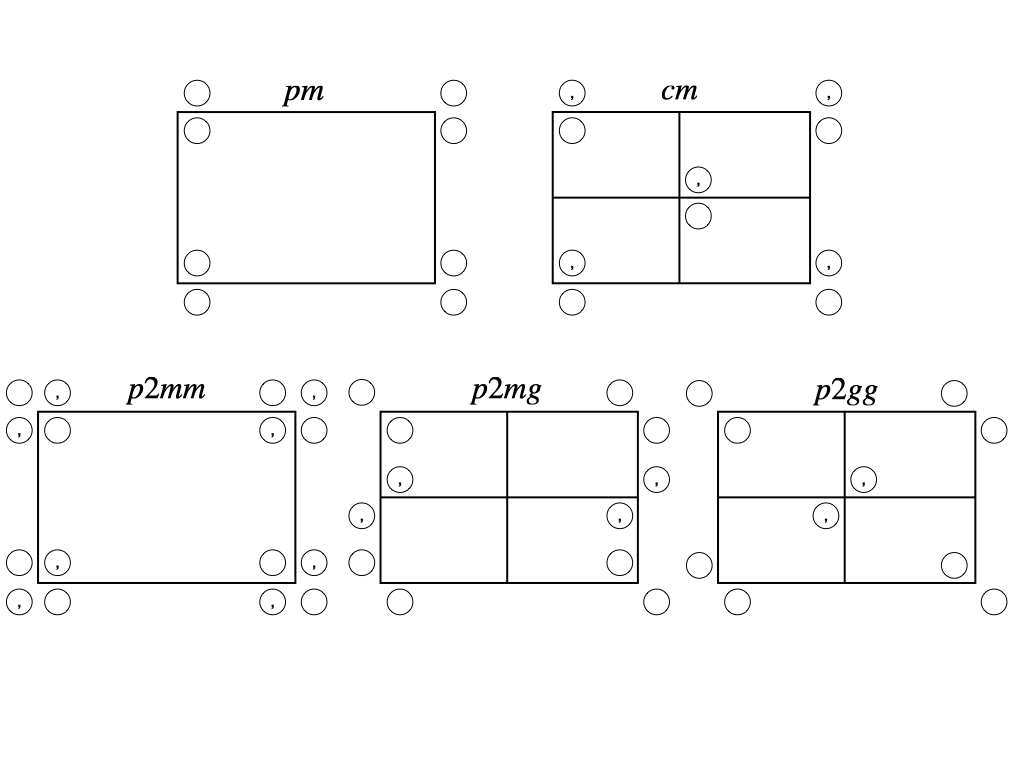
\includegraphics[width=0.9\textwidth]{figure/fig_plane_groups.png}
  \caption{Example diagrams of plane groups}
  \label{fig:plane-group-diagrams}
\end{figure}

% Primitive and centering

The plane group $pm$ is generated by the matrices
\begin{align*}
  % t(1, 0)
  \left(
    \begin{array}{cc|c}
        1 & 0 & 1 \\
        0 & 1 & 0 \\
        \hline
        0 & 0 & 1 \\
    \end{array}
  \right),
  % t(0, 1)
  \left(
    \begin{array}{cc|c}
        1 & 0 & 0 \\
        0 & 1 & 1 \\
        \hline
        0 & 0 & 1 \\
    \end{array}
  \right),
  % m
  \left(
    \begin{array}{cc|c}
        -1 & 0 & 0 \\
        0  & 1 & 0 \\
        \hline
        0 & 0 & 1 \\
    \end{array}
  \right),
\end{align*}
which correspond to $t(1, 0)$, $t(0, 1)$, and $m$ operations, respectively\footnote{
  Do not worry about the notations for symmetry operations such as $t(1, 0)$ or $m_{10}$.
  They are not required to read the remained document.
}.

The plane group $cm$ is generated by the matrices
\begin{align*}
  % t(1/2, 1/2)
  \left(
    \begin{array}{cc|c}
        1 & 0 & \frac{1}{2} \\
        0 & 1 & \frac{1}{2}\\
        \hline
        0 & 0 & 1 \\
    \end{array}
  \right),
  % t(1/2, -1/2)
  \left(
    \begin{array}{cc|c}
        1 & 0 & \frac{1}{2} \\
        0 & 1 & -\frac{1}{2}\\
        \hline
        0 & 0 & 1 \\
    \end{array}
  \right),
  % m
  \left(
    \begin{array}{cc|c}
        -1 & 0 & 0 \\
        0  & 1 & 0 \\
        \hline
        0 & 0 & 1 \\
    \end{array}
  \right),
\end{align*}
which correspond to $t(\frac{1}{2}, \frac{1}{2})$, $t(\frac{1}{2}, -\frac{1}{2})$, and $m$ operations, respectively.

% Symmorphic and nonsymmorphic

The plane group $p2mm$ is generated by the matrices,
\begin{align*}
  % t(1, 0)
  \left(
    \begin{array}{cc|c}
        1 & 0 & 1 \\
        0 & 1 & 0 \\
        \hline
        0 & 0 & 1 \\
    \end{array}
  \right),
  % t(0, 1)
  \left(
    \begin{array}{cc|c}
        1 & 0 & 0 \\
        0 & 1 & 1 \\
        \hline
        0 & 0 & 1 \\
    \end{array}
  \right),
  % 2
  \left(
    \begin{array}{cc|c}
        -1 & 0 & 0 \\
        0 & -1 & 0 \\
        \hline
        0 & 0 & 1 \\
    \end{array}
  \right),
  % m_01
  \left(
    \begin{array}{cc|c}
        -1 & 0 & 0 \\
        0 & 1 & 0 \\
        \hline
        0 & 0 & 1 \\
    \end{array}
  \right),
  % m_10
  \left(
    \begin{array}{cc|c}
        1 & 0 & 0 \\
        0 & -1 & 0 \\
        \hline
        0 & 0 & 1 \\
    \end{array}
  \right),
\end{align*}
which correspond to $t(1, 0)$, $t(0, 1)$, $2$, $m_{01}$, and $m_{10}$ operations, respectively.

The plane group $p2mg$ is generated by the matrices,
\begin{align*}
  % t(1, 0)
  \left(
    \begin{array}{cc|c}
        1 & 0 & 1 \\
        0 & 1 & 0 \\
        \hline
        0 & 0 & 1 \\
    \end{array}
  \right),
  % t(0, 1)
  \left(
    \begin{array}{cc|c}
        1 & 0 & 0 \\
        0 & 1 & 1 \\
        \hline
        0 & 0 & 1 \\
    \end{array}
  \right),
  % 2
  \left(
    \begin{array}{cc|c}
        -1 & 0 & 0 \\
        0 & -1 & 0 \\
        \hline
        0 & 0 & 1 \\
    \end{array}
  \right),
  % m_01
  \left(
    \begin{array}{cc|c}
        -1 & 0 & \frac{1}{2} \\
        0 & 1 & 0 \\
        \hline
        0 & 0 & 1 \\
    \end{array}
  \right),
  % a
  \left(
    \begin{array}{cc|c}
        1 & 0 & \frac{1}{2} \\
        0 & -1 & 0 \\
        \hline
        0 & 0 & 1 \\
    \end{array}
  \right),
\end{align*}
which correspond to $t(1, 0)$, $t(0, 1)$, $2$, $m$, and $a$ operations, respectively.

The plane group $p2gg$ is generated by the matrices,
\begin{align*}
  % t(1, 0)
  \left(
    \begin{array}{cc|c}
        1 & 0 & 1 \\
        0 & 1 & 0 \\
        \hline
        0 & 0 & 1 \\
    \end{array}
  \right),
  % t(0, 1)
  \left(
    \begin{array}{cc|c}
        1 & 0 & 0 \\
        0 & 1 & 1 \\
        \hline
        0 & 0 & 1 \\
    \end{array}
  \right),
  % 2
  \left(
    \begin{array}{cc|c}
        -1 & 0 & 0 \\
        0 & -1 & 0 \\
        \hline
        0 & 0 & 1 \\
    \end{array}
  \right),
  % b
  \left(
    \begin{array}{cc|c}
        -1 & 0 & \frac{1}{2} \\
        0 & 1 & \frac{1}{2} \\
        \hline
        0 & 0 & 1 \\
    \end{array}
  \right),
  % a
  \left(
    \begin{array}{cc|c}
        1 & 0 & \frac{1}{2} \\
        0 & -1 & \frac{1}{2} \\
        \hline
        0 & 0 & 1 \\
    \end{array}
  \right),
\end{align*}
which correspond to $t(1, 0)$, $t(0, 1)$, $2$, $b$, and $a$ operations, respectively.
